\begin{problem}{Mostrando grafos}{Standard input}{Standard output}{1 second}{}

% Original idea         
% Problem statement     
% Testset               

En la clase de algoritmos y estructuras de datos, el profesor estaba explicando el tema de árboles y Gerardo (uno de sus estudiantes) lo interrumpió para preguntar que tipos de recorridos en árboles existían. Como faltaban 5 minutos para el final, el profesor decidió dejarles de tarea hacer un algoritmo que recorra un árbol por niveles.

Dado que ya no tenía mucho tiempo para explicar todos los detalles dejó en la pizarra  la siguiente explicación sobre un árbol:

Un \'arbol $ T = (V, E)$ está conformado por un conjunto de nodos $V = \lbrace 0, 1, \dots, N-1\rbrace$, y un conjunto de aristas $E = \lbrace (p, q) / p, q \in V \rbrace$. El árbol tiene un nodo ra\'iz $r \in V$ y tiene exáctamente $N-1$ aristas. Cada elemento $(p, q) \in E$, indicar\'a que existe arista desde el nodo $p$ hacia el nodo $q$.

Además, considerando el siguiente conjunto de nodos $V = \lbrace 0, 1, 2, 3, 4, 5, 6, 7, 8, 9, 10, 11 \rbrace$ y el conjunto de aristas $E=\lbrace(4,3), (4, 6), (4, 0), (3, 1), (3, 7), (3, 9), (6, 2), (6, 8), (0, 11), (1, 5), (1, 10)\rbrace$, se puede determinar que la raíz del árbol es el nodo $4$ y el árbol tiene $4$ niveles. Sin embargo, es posible formar diferentes árboles dependiendo del órden en el que se procesen los nodos. Por ejemplo, con esas aristas pueden formarse los dos árboles siguientes:

\begin{figure}[h]
\centering
  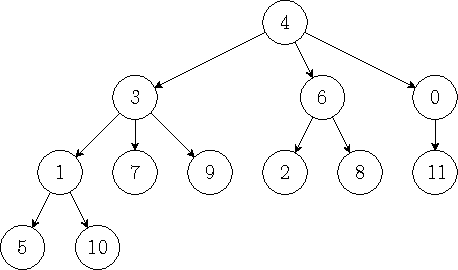
\includegraphics[width=9cm]{images/tree.pdf}
  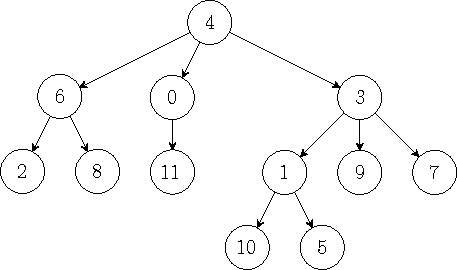
\includegraphics[width=9cm]{images/tree2.pdf}
  \caption{Dos árboles que pueden armados considerando la configuración explicada en el párrafo anterior.}
\end{figure}

Tu deber es armar un árbol y recorrerlo por niveles. Es decir, considerando el árbol  que aparece en la parte superior, primero se muestra la raiz (nodo 4), luego sus hijos (nodos 3, 6, y 0), después los hijos de estos nodos que se encuentran en el siguiente nivel (nodos 1, 7, 9, 2, 8, y 11), y as\'i sucesivamente. Por consiguiente, la respuesta que se busca ser\'ia la siguiente:

\begin{verbatim}
      4
      3 6 0
      1 7 9 2 8 11
      5 10
\end{verbatim}

Pero dependiendo de como se arme el árbol se pueden tener varias respuestas válidas. Para nuestro ejemplo, otra respuesta válida considerando el árbol inferior es:

\begin{verbatim}
      4
      6 0 3
      2 8 11 1 9 7
      10 5
\end{verbatim}

\InputFile

La entrada del problema contiene varios casos de prueba. La primera línea es un entero $T$ $(1 \leq T \leq 100)$ indicando el número de casos de prueba. Cada caso de prueba sigue el siguiente formato de entrada:

\begin{itemize}
\item La primera línea contiene un entero $N$ indicando la cantidad de nodos del árbol ($1 \leq N \leq 10^3$).

\item La segunda línea contiene $N - 1$ pares de enteros $p, q$ representando las aristas del árbol ($0 \leq p, q < N, p\neq q$). Por claridad, un par de enteros $p, q$ expresa una arista del nodo $p$ hacia el nodo $q$.

\end{itemize}

\OutputFile
Para cada caso de prueba, el programa deber\'a imprimir ``\texttt{Caso \#i:}'' (sin comillas) y a partir de la siguiente linea el árbol por niveles. Como pueden haber varios recorridos por niveles válidos para un mismo conjunto de aristas, imprimir cualquier recorrido válido.

\Example

\begin{example}
\exmp{%%INPUT
3
2
0 1
5
0 1 1 2 2 3 3 4
12
4 3 3 1 6 2 0 11 3 9 4 0 1 5 6 8 1 10 3 7 4 6%%END-INPUT
}{ %%OUTPUT
Caso \#1:
0
1
Caso \#2:
0
1
2
3
4
Caso \#3:
4
3 6 0
1 7 9 2 8 11
5 10
} %%END-OUTPUT
\end{example}

\end{problem}
